\vfill
\pagebreak
\chapter{Resultado}
En esta secci�n se presentan los resultados obtenidos al aplicar las t�cnicas de data discovery para realizar un an�lisis de las informaciones, cruzarlos, georeferenciarlos, encontrar l�neas de tendencias y pron�sticos de crecimiento a futuro tanto del consumo de energ�a, de clientes de la ANDE y de la poblaci�n del pa�s. En cada caso se presenta un an�lisis que demuestra con gr�ficos intuitivos que en ciertas ocasiones no existe una relaci�n proporcional entra algunas dimensiones.
\section{Aplicaci�n de Data Discovery a datos de instituciones del Estado}



Generalmente las organizaciones no logran comprender en su totalidad los datos que generan. La consecuencia de no comprender esos datos puede resultar en la mala toma de decisi�n, lo cual podr�a ocasionar un gran impacto negativo a la organizaci�n. La informaci�n es considerada como uno de los recursos m�s importantes en una organizaci�n, y en base a esta informaci�n, se puede obtener conocimiento que podr�a ayudar a obtener mejores resultados.

En el presente trabajo son analizados datos de la ANDE y de la DGEEC, relacionando ambos conjuntos de datos, con el objetivo de obtener informaci�n de inter�s para la organizaci�n.


\section{Datos de la ANDE y de la DGEEC}

Se cuenta con datos de consumo de energ�a el�ctrica, facturaciones, grupos de consumo (residencial, industrial, exportaci�n, comercial, gubernamental y otros), por a�o (2000-2014), por departamento y distrito. Estos datos fueron solicitados formalmente a la instituci�n por medio de la Facultad de Ciencias y Tecnolog�a de la Universidad Cat�lica, a la cual tuvimos una respuesta favorable.

\section{Dashboard de control / monitoramiento}

En esta secci�n se presentan 4 productos construidos en esta Tesis, los cuales son Paneles de Control, en donde se relacionan conjuntos de datos de la ANDE y de la DGEEC. Una de las t�cnicas utilizadas para medir el crecimiento es la tasa de crecimiento, la cual se obtiene de la siguiente forma:

Es calculado el porcentaje de crecimiento ocurrido por cada a�o (Ej: Si al cerrar el a�o 2014, la cantidad de clientes fue de 1.000.000 y en el a�o 2015 aument� 100.000, esto quiere decir que en el a�o 2015, la tasa de crecimiento de los clientes fue del 10\%, es decir, hubo un crecimiento positivo y la cantidad de clientes ha aumentado). Suponiendo que en el a�o 2016 la ANDE cierra con un total de 1.000.000 de clientes, su crecimiento ser a 10\% menor al a�o anterior. La f�rmula empleada (ver f�rmula Tasa de variaci�n abajo), donde n es el a�o actual y n-1 el a�o anterior, PIB indica la cantidad de clientes que posee la ANDE .

\begin{mycapequ}[!ht]
	\caption{F�rmula: Tasa de variaci�n}
	\begin{equation}
		t_n = \cfrac{PIB_n - PIB_{n-1}}{PIB_{n-1}} \times 100 \nonumber
	\end{equation}
	\begin{center}
		Fuente: \cite{rudiger2002macroeconomia}
	\end{center}	
\end{mycapequ}


\subsection{Dashboard - Clientes Facturados vs Crecimiento Poblacional}

En el dashboard de la Figura ~\ref{fig:ClientesFacturadosVsCrecimientoPoblacional3} son utilizados datos hist�ricos de la poblaci�n, prove�dos por la \gls{sig:DGEEC}, y datos de clientes, tales como el consumo y facturaci�n, prove�dos por la \gls{sig:ANDE}. Es importante notar en la figura, que independiente a que la tasa de crecimiento poblacional se mantenga casi constante, la tasa de crecimiento del consumo se eleva de forma pronunciada. Adem�s, puede ser muy relevante la informaci�n de proyecci�n del consumo para los pr�ximos a�os, para elaborar una planificaci�n en la ampliaci�n de la capacidad de transmisi�n o distribuci�n de energ�a.

\textsc{\begin{figure}[H]
	\centering
	\caption{Clientes Facturados vs Crecimiento Poblacional}
	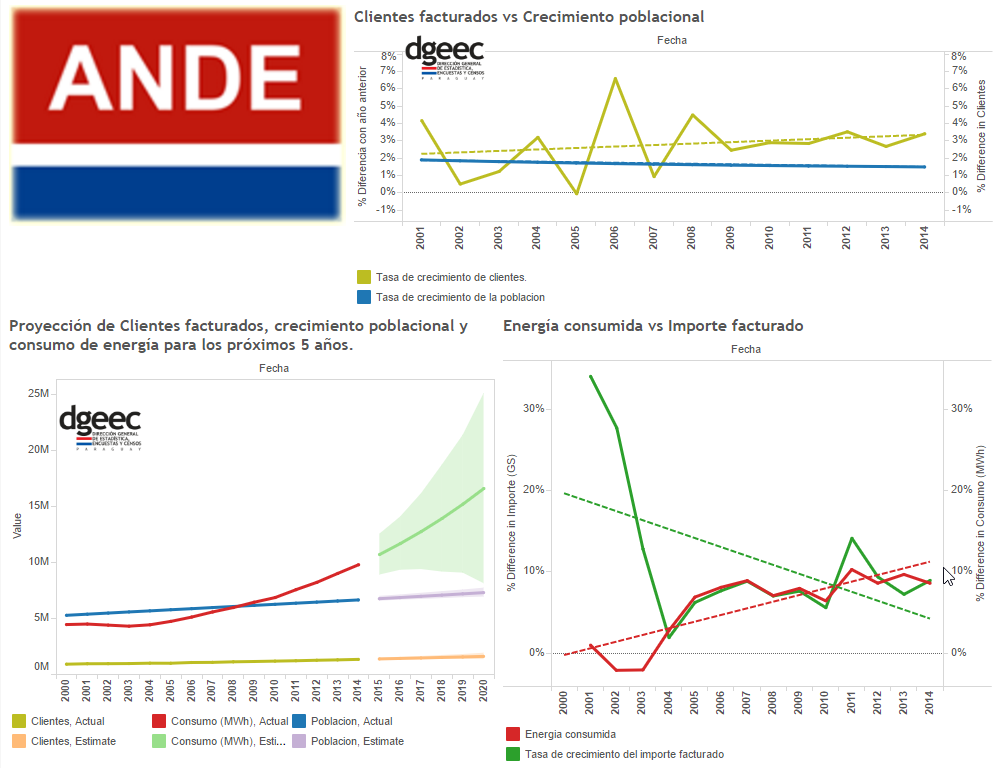
\includegraphics[width=\linewidth]{imagenes/ClientesFacturadosVsCrecimientoPoblacional3}
	\caption*{Fuente: Elaboraci�n propia.}
	\label{fig:ClientesFacturadosVsCrecimientoPoblacional3}
\end{figure}}


En la Figura ~\ref{fig:ClientesFacturadosVsCrecimientoPoblacional4} se presentan dos tasas de crecimiento: de Clientes de la ANDE y de la Poblaci�n del Paraguay. Es importante notar que el ritmo de crecimiento de la poblaci�n disminuye con el tiempo, pero no as� el ritmo de consumo de electricidad. No existe una relaci�n directa entre estas dos tasas por el momento, lo cual puede deberse a factores tales como instalaci�n de mayor cantidad de dispositivos el�ctricos en residencias, o bien la instalaci�n de m�s industrias las cuales tienen un alto nivel de consumo de electricidad. Es importante notar que la tendencia de la tasa de crecimiento del consumo de electricidad es positiva, lo cual podr�a ayudar a planificar una mayor inversi�n en la red de electricidad para aquellas zonas donde se registran tendencias mayores al consumo.

\textsc{\begin{figure}[H]
	\centering
	\caption{Clientes Facturados vs Crecimiento Poblacional}
	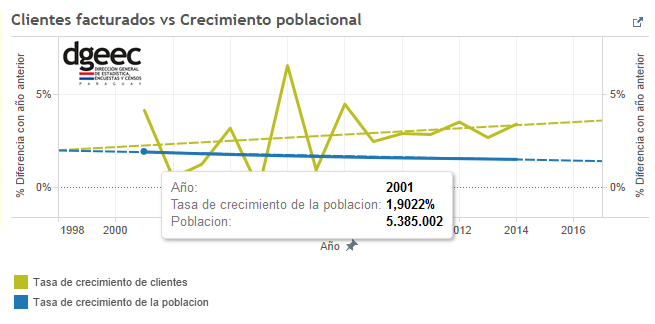
\includegraphics[width=\linewidth]{imagenes/ClientesFacturadosVsCrecimientoPoblacional4}
	\caption*{Fuente: Elaboraci�n propia.}
	\label{fig:ClientesFacturadosVsCrecimientoPoblacional4}
\end{figure}}


En la figura ~\ref{fig:ClientesFacturadosVsCrecimientoPoblacional} observamos que la cantidad de la poblaci�n en el a�o 2002 cerr� con un total de 5.484.610, la cual su crecimiento fue del 1,8497\% que equivale a 99608.

\textsc{\begin{figure}[H]
	\centering
	\caption{Clientes Facturados vs Crecimiento Poblacional}
	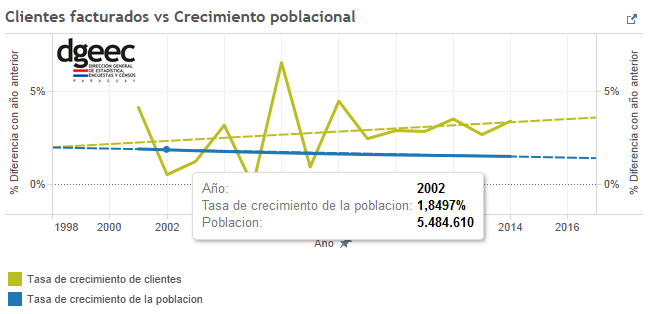
\includegraphics[width=\linewidth]{imagenes/ClientesFacturadosVsCrecimientoPoblacional}
	\caption*{Fuente: Elaboraci�n propia.}
	\label{fig:ClientesFacturadosVsCrecimientoPoblacional}
\end{figure}}


En la figura ~\ref{fig:ClientesFacturadosVsCrecimientoPoblacional2} se muestran valores que representan el porcentaje del crecimiento de los clientes de la ANDE. Como podemos ver, hay a�os en que el aumento es muy evidente (2004,2006,2008) y hay a�os en que este es m�nimo(2002,2005,2007). Las l�neas discontinuas representan las tendencias de ambos puntos. Por ejemplo, la cantidad de clientes en el a�o 2001 fue de 959.580, la cual aument� el 4.1\% respecto al a�o anterior.

\textsc{\begin{figure}[H]
	\centering
	\caption{Clientes Facturados vs Crecimiento Poblacional}
	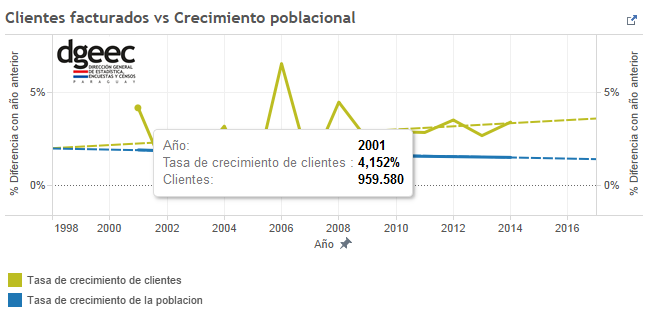
\includegraphics[width=\linewidth]{imagenes/ClientesFacturadosVsCrecimientoPoblacional2}
	\caption*{Fuente: Elaboraci�n propia.}
	\label{fig:ClientesFacturadosVsCrecimientoPoblacional2}
\end{figure}}


En la figura ~\ref{fig:ClientesFacturadosVsCrecimientoPoblacional5}, se muestra la cantidad de clientes correspondiente al a�o 2002, vemos que ascendi� a 964.449 con un aumento de 4.869, que corresponde a un incremento del 0.5\% respecto  al a�o 2001. Sin embargo en la figura ~\ref{fig:ClientesFacturadosVsCrecimientoPoblacional6}, en el a�o 2003 el incremento fue de 1.2\%, la cual representa a un aumento de m�s que el doble del a�o anterior llegando a aumentar 11830 clientes.

\textsc{\begin{figure}[H]
	\centering
	\caption{Clientes Facturados vs Crecimiento Poblacional}
	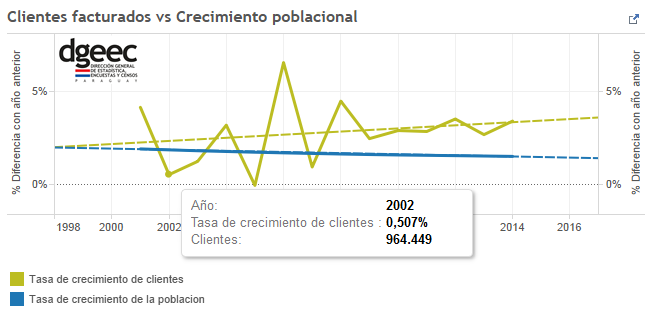
\includegraphics[width=\linewidth]{imagenes/ClientesFacturadosVsCrecimientoPoblacional5}
	\caption*{Fuente: Elaboraci�n propia.}
	\label{fig:ClientesFacturadosVsCrecimientoPoblacional5}
\end{figure}}

\textsc{\begin{figure}[H]
	\centering
	\caption{Clientes Facturados vs Crecimiento Poblacional}
	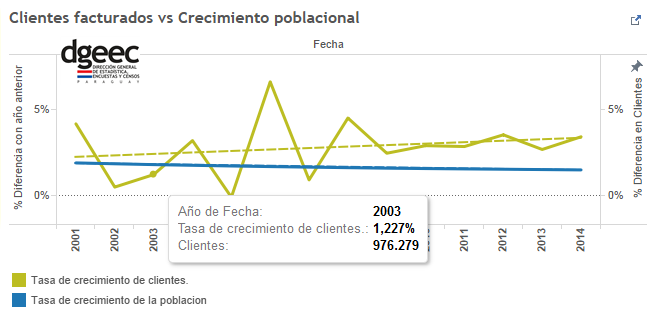
\includegraphics[width=\linewidth]{imagenes/ClientesFacturadosVsCrecimientoPoblacional6}
	\caption*{Fuente: Elaboraci�n propia.}
	\label{fig:ClientesFacturadosVsCrecimientoPoblacional6}
\end{figure}}

En la figura ~\ref{fig:ProyeccionDeClientesFacturadosCrecimientoPoblacionalYConsumoDeEnergiaParaLosProximos5Anos} se puede observar con m�s detalle la proyecci�n (forecasting) del consumo, crecimiento poblacional y cantidad de clientes. Se puede notar que existe una mayor probabilidad que en promedio, el consumo de electricidad aumente de forma considerable hasta el 2020 (l�nea roja). Adem�s, este aumento es mayor en proporci�n al aumento de la poblaci�n y a la cantidad de clientes.

Esto demuestra claramente que el consumo aumenta cada vez m�s, independiente que se d� un aumento en la misma proporci�n de clientes o poblaci�n. Esto puede ocurrir a causa de varios factores, entre ellos, el aumento de dispositivos el�ctricos en las residencias, debido al aumento en la capacidad adquisitiva de las personas. Tambi�n se puede dar a causa de un aumento en la cantidad de industrias.

\textsc{\begin{figure}[H]
	\centering
	\caption{Proyecci�n de Clientes Facturados Crecimiento Poblacional Y Consumo De Energ�a para los Pr�ximos 5 A�os}
	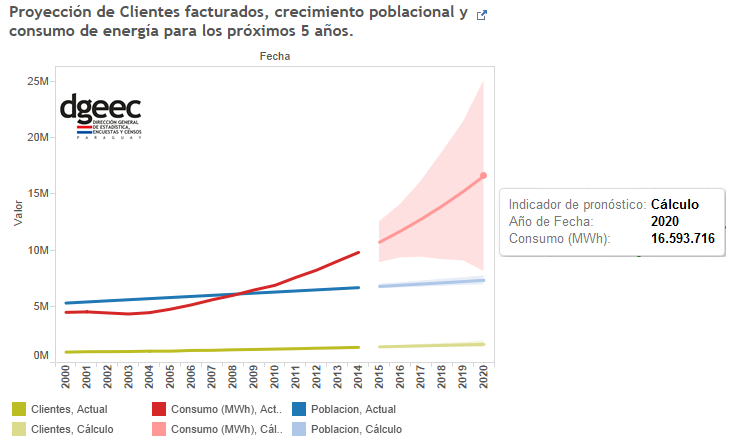
\includegraphics[width=\linewidth]{imagenes/ProyeccionDeClientesFacturadosCrecimientoPoblacionalYConsumoDeEnergiaParaLosProximos5Anos}
	\caption*{Fuente: Elaboraci�n propia.}
	\label{fig:ProyeccionDeClientesFacturadosCrecimientoPoblacionalYConsumoDeEnergiaParaLosProximos5Anos}
\end{figure}}

En el tercer y �ltimo gr�fico de este panel, se muestra el porcentaje del crecimiento anual de los importes facturados y consumo de energ�a. Se puede observar que la facturaci�n de la ANDE, en general es proporcional al consumo de energ�a el�ctrica, excepto en el a�o 2011 (Figura ~\ref{fig:EnergiaConsumidaVsImporteFacturado3}), en la cual el importe facturado fue superior al aumento del consumo de energ�a. Sin embargo, en el a�o 2013 (Figura ~\ref{fig:EnergiaConsumidaVsImporteFacturado2}) se registra nuevamente un aumento en relaci�n a a�os anteriores.

\textsc{\begin{figure}[H]
	\centering
	\caption{Energ�a Consumida vs Importe Facturado}
	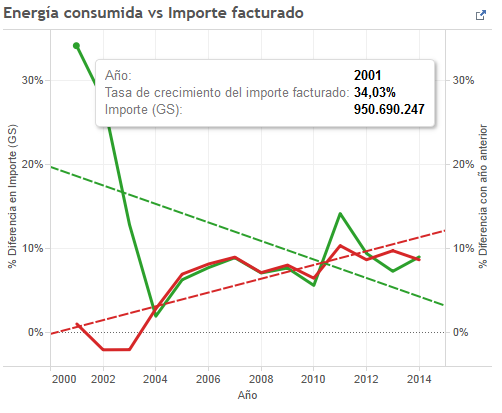
\includegraphics[width=\linewidth]{imagenes/EnergiaConsumidaVsImporteFacturado}
	\caption*{Fuente: Elaboraci�n propia.}
	\label{fig:EnergiaConsumidaVsImporteFacturado3}
\end{figure}}

\textsc{\begin{figure}[H]
	\centering
	\caption{Energ�a Consumida vs Importe Facturado}
	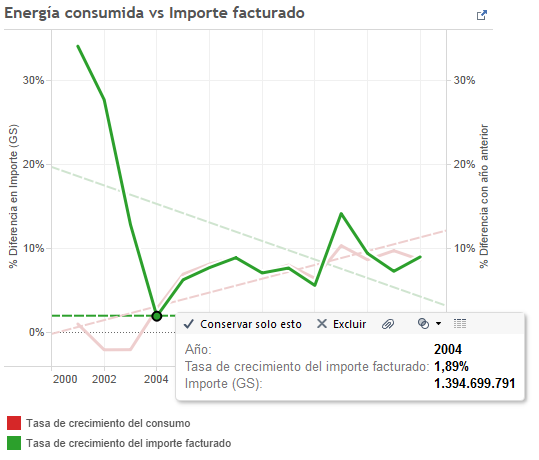
\includegraphics[width=\linewidth]{imagenes/EnergiaConsumidaVsImporteFacturado2}
	\caption*{Fuente: Elaboraci�n propia.}
	\label{fig:EnergiaConsumidaVsImporteFacturado2}
\end{figure}}

\subsection{Panel estad�stico de consumo de electricidad por sector}

En la figura ~\ref{fig:EstadisticaDeConsumoDeElectricidadPorSector1990-2014} se presenta un gr�fico con el consumo de energ�a hist�rica, que abarca desde el a�o 1990 hasta 2014. Estos datos est�n clasificados por los siguientes criterios de la ANDE: Alumbrado P�blico, Comercial, Exportaci�n, Gubernamental, Industrial y Residencial. En este gr�fico se puede apreciar que el mayor consumo de energ�a se encuentra en el sector Residencial. Sin embargo, los valores de Exportaci�n de energ�a fue disminuyendo durante el tiempo. Esto tiene sentido debido a que ambos valores son inversamente proporcionales, esto es, cuando el consumo nacional se incrementa, se hace un mayor uso de energ�a en el pa�s, por lo tanto disminuye la energ�a disponible para exportaci�n.

\textsc{\begin{figure}[H]
	\centering
	\caption{Estad�stica de consumo de electricidad por sector(1990-2014)}
	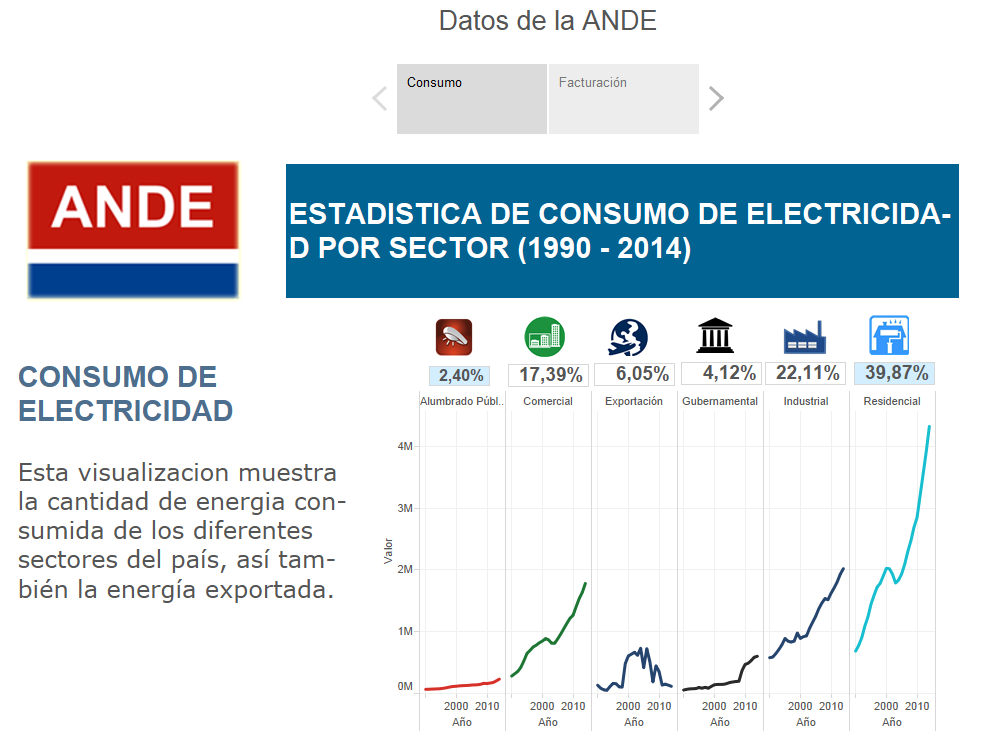
\includegraphics[width=\linewidth]{imagenes/EstadisticaDeConsumoDeElectricidadPorSector1990-2014}
	\caption*{Fuente: Elaboraci�n propia.}
	\label{fig:EstadisticaDeConsumoDeElectricidadPorSector1990-2014}
\end{figure}}

\noindent
La Figura ~\ref{fig:ImporteFacturadoPorAnoYSector1990-2014} presenta las informaciones de facturaci�n tambi�n clasificados por sector, con el recurso de filtros por a�o. Es importante destacar un factor resaltante: aunque energ�a exportada disminuy�, el valor facturado por energ�a vendida al exterior aument�. Es probable que esto se haya debido al aumento de la tarifa de energ�a vendida, lo cual beneficia al pa�s.

\textsc{\begin{figure}[H]
	\centering
	\caption{Importe facturado por a�o y sector(1990-2014)}
	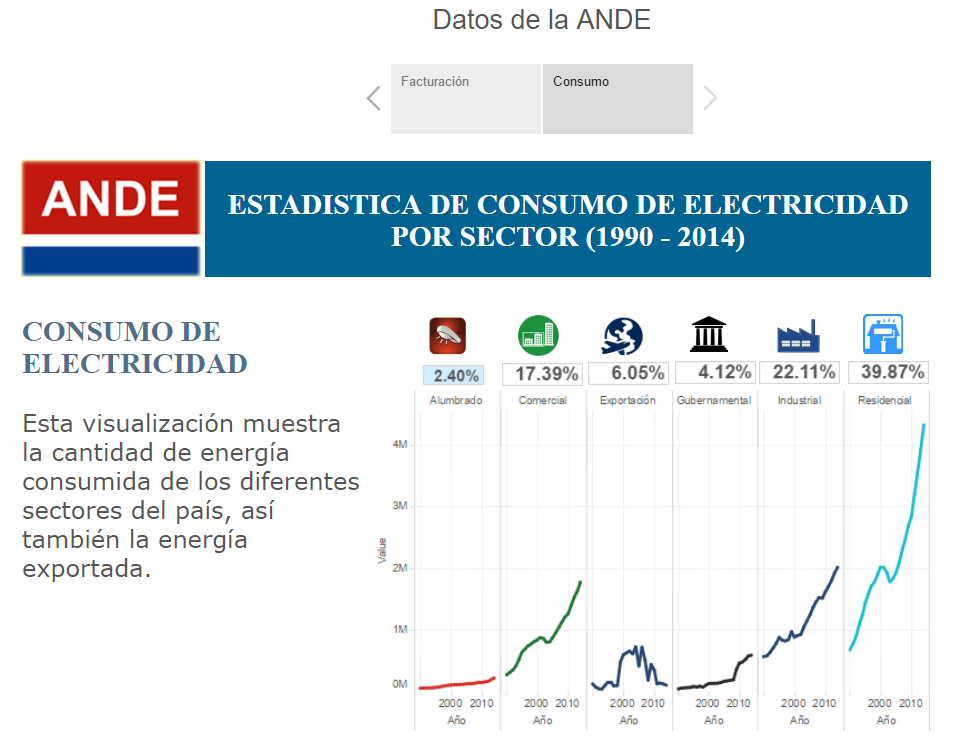
\includegraphics[width=\linewidth]{imagenes/ImporteFacturadoPorAnoYSector1990-2014}
	\caption*{Fuente: Elaboraci�n propia.}
	\label{fig:ImporteFacturadoPorAnoYSector1990-2014}
\end{figure}}

\subsection{Panel comparativo de Tasa de crecimiento y el Consumo de energ�a}

En la figura ~\ref{fig:TasaDeCrecimientoVsConsumoDeEnergia} se presenta un panel comparativo entre la tasa de crecimiento de clientes y consumo de energ�a. Tambi�n se cuenta con un mapa para filtrar por regi�n del pa�s. 

\textsc{\begin{figure}[H]
	\centering
	\caption{Tasa de crecimiento vs Consumo de energ�a}
	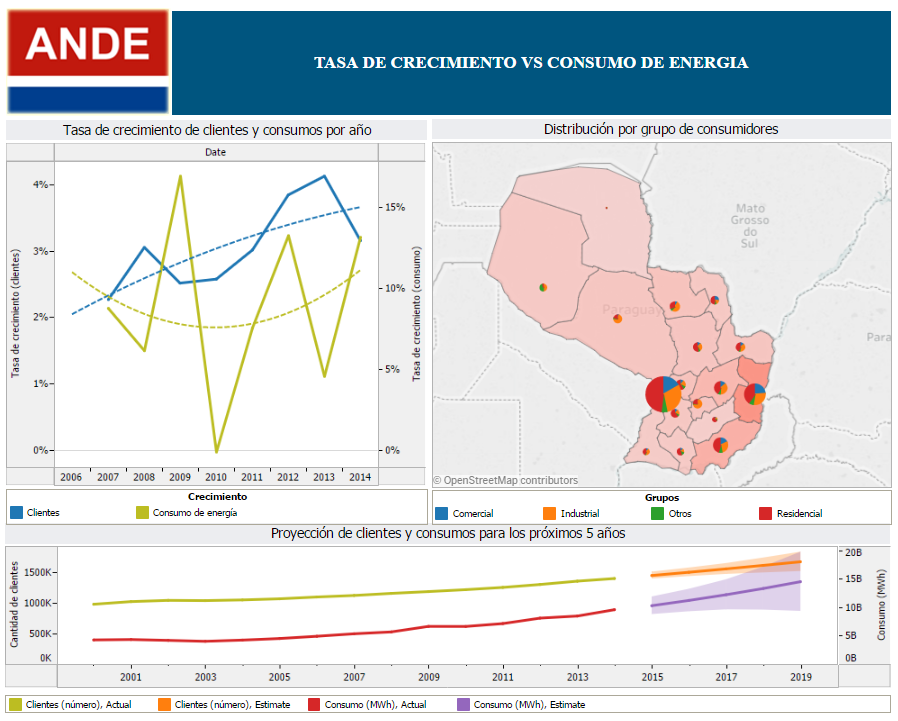
\includegraphics[width=\linewidth]{imagenes/TasaDeCrecimientoVsConsumoDeEnergia}
	\caption*{Fuente: Elaboraci�n propia.}
	\label{fig:TasaDeCrecimientoVsConsumoDeEnergia}
\end{figure}}


En el gr�fico situado a la derecha del mapa (Figura ~\ref{fig:TasaDeCrecimientoVsConsumoDeEnergia2}), se tiene el consumo y crecimiento de clientes. Para un mejor an�lisis fue necesario suavizar los datos calculando lineas de tendencia, debido a una inestabilidad de los datos de consumo. As� se puede apreciar, que existe una tendencia de crecimiento sostenido durante el tiempo de clientes. Sin embargo, la tendencia que el consumo crezca es mayor al de clientes.

\textsc{\begin{figure}[H]
	\centering
	\caption{Tasa de crecimiento vs Consumo de energ�a, filtrado por el departamento Alto Paran�}
	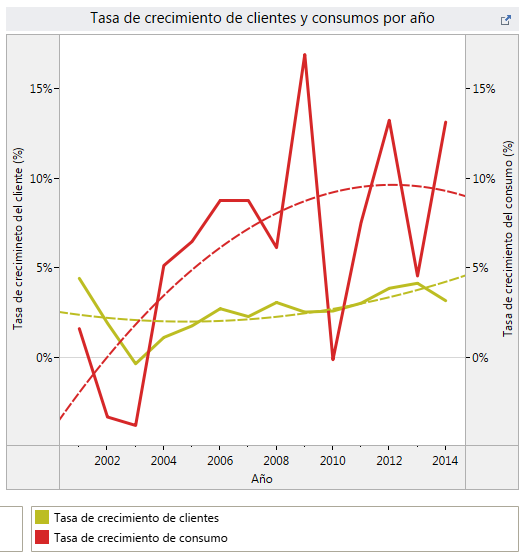
\includegraphics[width=\linewidth]{imagenes/TasaDeCrecimientoVsConsumoDeEnergia2}
	\caption*{Fuente: Elaboraci�n propia.}
	\label{fig:TasaDeCrecimientoVsConsumoDeEnergia2}
\end{figure}}


Debajo se presenta un cuadro con la l�nea de cada valor (Figura ~\ref{fig:ProyeccionDeClientesYConsumosParaLosProximos5Anos}), de crecimiento y consumo. Con el uso de un recurso disponible que cuenta la herramienta escogida Tableau, es posible realizar an�lisis predictivo  (forecasting) del crecimiento y consumo. Tableau utiliza un algoritmo llamado Suavizado Exponencial, muy conocido en el �rea de Matem�ticas Estad�sticas. En este gr�fico se puede notar que existe una mayor probabilidad que en los pr�ximos a�os aumente considerablemente el consumo, superando su media. Sin embargo, se nota que el ritmo de crecimiento de clientes es sostenible, y no tiene una alta probabilidad de sufrir un aumento abrupto.

\textsc{\begin{figure}[H]
		\centering
		\caption{Proyecci�n de clientes y consumos para los pr�ximos 5 a�os}
		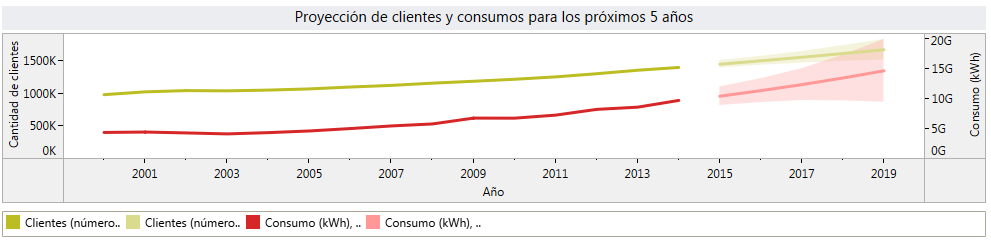
\includegraphics[width=\linewidth]{imagenes/ProyeccionDeClientesYConsumosParaLosProximos5Anos}
		\caption*{Fuente: Elaboraci�n propia.}
		\label{fig:ProyeccionDeClientesYConsumosParaLosProximos5Anos}
	\end{figure}}

	
\subsection{Panel de Tasa de crecimiento poblacional y Consumo de energ�a anual}

\textsc{\begin{figure}[H]
	\centering
	\caption{Panel de Tasa de crecimiento poblacional y Consumo de energ�a anual}
	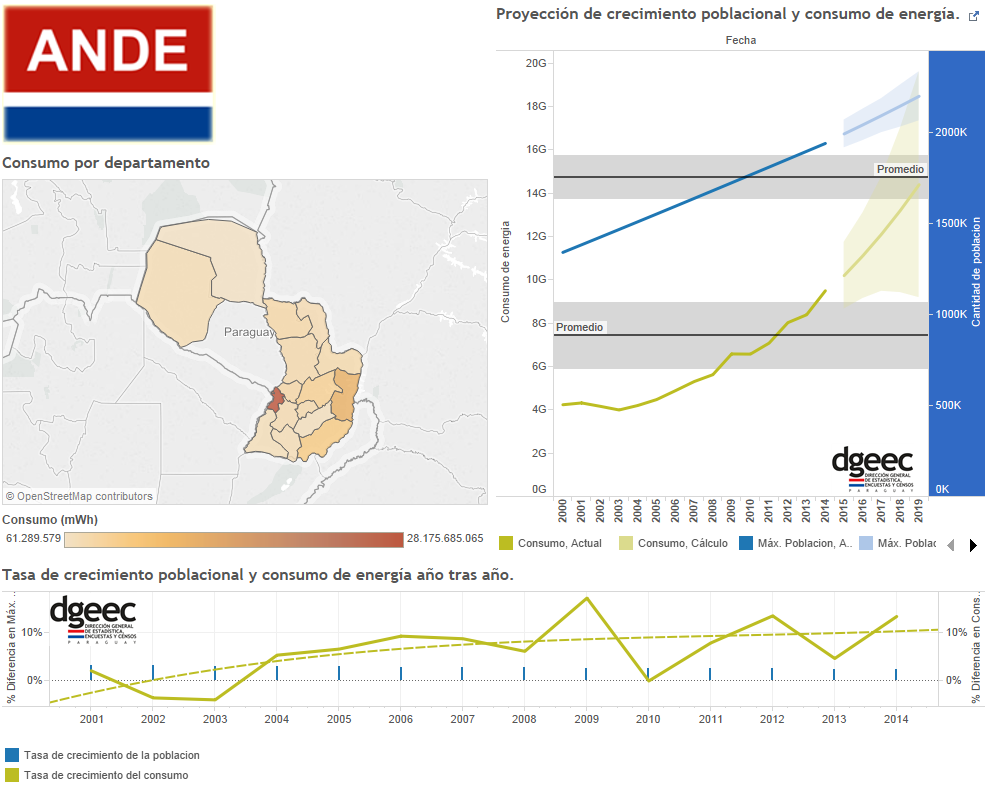
\includegraphics[width=\linewidth]{imagenes/TasaDeCrecimientoPoblacionalYConsumoDeEnergiaAnoTrasAno}
	\caption*{Fuente: Elaboraci�n propia.}
	\label{fig:TasaDeCrecimientoPoblacionalYConsumoDeEnergiaAnoTrasAno}
\end{figure}}

En la figura~\ref{fig:TasaDeCrecimientoPoblacionalYConsumoDeEnergiaAnoTrasAnoMapa} se presenta el panel comparativo de datos de crecimiento poblacional de la DGEEC y de consumo de la ANDE. En el mapa, cuando el color es m�s oscuro el consumo de energ�a es mayor, y si el color es m�s claro, el consumo es menor. Se puede notar que los departamentos Central y Alto Paran� son los que tiene mayor consumo de energ�a. 
Este tipo de gr�fico es muy �til cuando se desea analizar informaci�n de forma general y georeferenciada. Al ubicar el mouse sobre cualquier departamento, se presenta una ventana emergente indicando el valor de consumo del departamento seleccionado. Al seleccionar un departamento del mapa, los dem�s gr�ficos tambi�n se actualizan filtrando el departamento seleccionando. 

\textsc{\begin{figure}[H]
	\centering
	\caption{Consumo por departamento}
	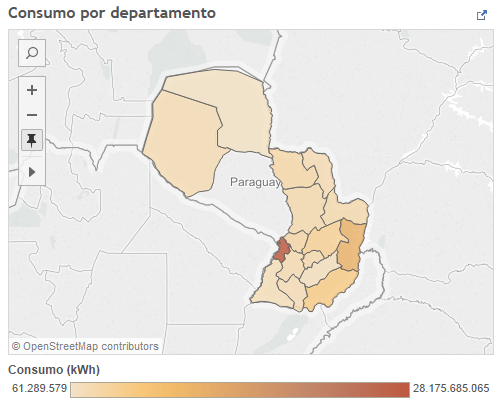
\includegraphics[width=\linewidth]{imagenes/TasaDeCrecimientoPoblacionalYConsumoDeEnergiaAnoTrasAnoMapa}
	\caption*{Fuente: Elaboraci�n propia.}
	\label{fig:TasaDeCrecimientoPoblacionalYConsumoDeEnergiaAnoTrasAnoMapa}
\end{figure}}

\noindent
 Los gr�ficos situados a la derecha y debajo del mapa presentan la tasa de crecimiento poblacional y de consumo de energ�a. Es importante notar que la tasa de crecimiento de la poblaci�n es casi constante, esto es, no tiene una gran variaci�n en el tiempo, ni una tendencia a alejarse de la media. Sin embargo, la tasa de crecimiento de consumo tiene una l�nea de tendencia a crecer durante el tiempo. As� puede apreciarse que, el consumo de energ�a no tiene una relaci�n de proporcionalidad con respecto al crecimiento de la poblaci�n.

\textsc{\begin{figure}[H]
	\centering
	\caption{Proyecci�n de crecimiento poblacional y consumo ee energ�a}
	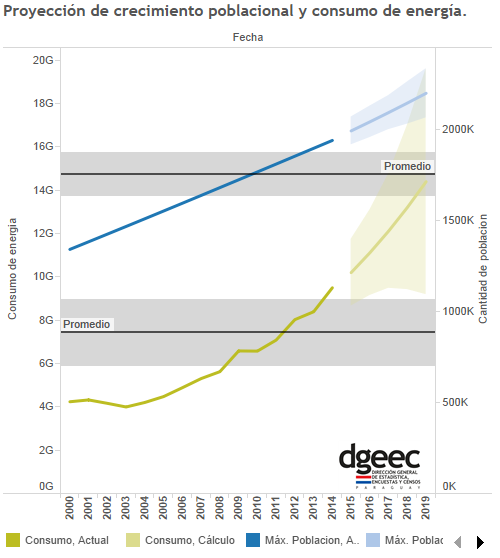
\includegraphics[width=\linewidth]{imagenes/ProyeccionDeCrecimientoPoblacionalYConsumoDeEnergia}
	\caption*{Fuente: Elaboraci�n propia.}
	\label{fig:ProyeccionDeCrecimientoPoblacionalYConsumoDeEnergia}
\end{figure}}

\noindent
En este gr�fico,  se muestra la misma informaci�n que el gr�fico anterior pero con diferente perspectiva, en este caso se calcula el porcentaje de crecimiento anual tanto de la poblaci�n, as� como del consumo.

\textsc{\begin{figure}[H]
	\centering
	\caption{Tasa de crecimiento poblacional y consumo de energ�a a�os tras a�os}
	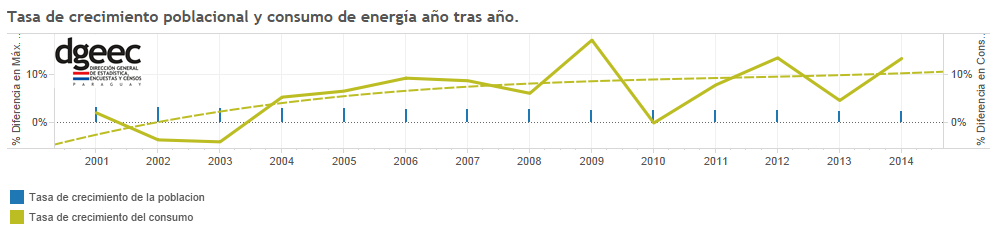
\includegraphics[width=\linewidth]{imagenes/ProyeccionDeClientesYConsumosParaLosProximos5Anos2}
	\caption*{Fuente: Elaboraci�n propia.}
	\label{fig:ProyeccionDeClientesYConsumosParaLosProximos5Anos2}
\end{figure}}


